% Oblique Incidence with using basics instructions
% Author: Edgar Fuentes (Club de LaTeX UC member)
\documentclass[border=5pt]{standalone}


\usepackage{tikz}
\usetikzlibrary{%
    decorations.pathreplacing,%
    decorations.pathmorphing%
}
\usepackage{verbatim}

\begin{comment}
:Title: Oblique Incidence
:Tags: Decorations, Physics & chemistry

Reflection and refraction of electromagnetic waves incident obliquely at plane interface. 

:Author: `Edgar Fuentes`_

.. _Edgar Fuentes: http://groups.google.co.ve/group/LaTeXuC

\end{comment}


\begin{document}
\pagestyle{empty}

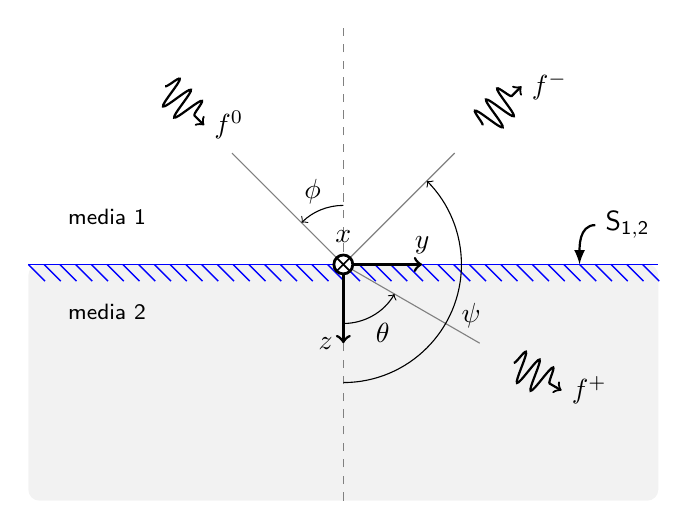
\begin{tikzpicture}[
    media/.style={font={\footnotesize\sffamily}},
    wave/.style={
        decorate,decoration={snake,post length=1.4mm,amplitude=2mm,
        segment length=2mm},thick},
    interface/.style={
        % The border decoration is a path replacing decorator. 
        % For the interface style we want to draw the original path.
        % The postaction option is therefore used to ensure that the
        % border decoration is drawn *after* the original path.
        postaction={draw,decorate,decoration={border,angle=-45,
                    amplitude=0.3cm,segment length=2mm}}},
    ]
    % Round rectangle
    \fill[gray!10,rounded corners] (-4,-3) rectangle (4,0);
    % Interface
    \draw[blue,line width=.5pt,interface](-4,0)--(4,0);
    % Vertical dashed line
    \draw[dashed,gray](0,-3)--(0,3);
    % Coordinates system
    \draw(0,0.15)node[above]{$x$};
    \draw[<->,line width=1pt] (1,0) node[above]{$y$}-|(0,-1) node[left]{$z$};
    % Incidence
    \draw[->,wave]
         (135:3.2cm)--(135:2.5cm)node[right]{$f^0$};
    \draw[gray](0:0cm)--(135:2cm);
    \path (0,0)++(113:1cm)node{$\phi$};
    \draw[->](0,0.75)arc(90:135:.75cm);
    % Transmission
    \draw[->,wave]
         (-30:2.5cm)--(-30:3.2cm)node[right]{$f^+$};
    \draw[gray](0:0cm)--(-30:2cm);
    \path (0,0)++(-60:1cm)node{$\theta$};
    \draw[->] (0,-0.75) arc (-90:-30:.75cm);
    % Reflection
    \draw[->,wave]
         (45:2.5cm)--(45:3.2cm)node[right]{$f^-$};
    \path (0,0)++(-22:1.75cm) node{$\psi$};
    \draw[gray](0:0cm)--(45:2cm);
    \draw[->] (0,-1.5)arc(-90:45:1.5cm);
    % Media names
    \path[media] (-3,.6)  node {media 1}
                 (-3,-.6) node {media 2};

    % $x$ axis
    \filldraw[fill=white,line width=1pt](0,0)circle(.12cm);
    \draw[line width=.6pt] (0,0)
                          +(-135:.12cm) -- +(45:.12cm)
                          +(-45:.12cm) -- +(135:.12cm);
    % Interface pointer
    \draw[-latex,thick](3.2,0.5)node[right]{$\mathsf{S_{1,2}}$}
         to[out=180,in=90] (3,0);
    % To-paths are really useful for drawing curved lines. The above
    % to path is equal to:
    %
    % \draw[-latex,thick](3.2,0.5)node[right]{$\mathsf{S_{1,2}}$}
    %      ..controls +(180:.2cm) and +(up:0.25cm) .. (3,0);
    % Internally the to path is translated to a similar bezier curve,
    % but the to path syntax hides the complexity from the user. 
\end{tikzpicture}


\end{document}
